\documentclass[11pt]{article}
\usepackage[a4paper, total={6in, 8in}]{geometry}
\usepackage{amsmath}
\usepackage{amsthm}
\usepackage{graphicx}
\usepackage{amsfonts}
\usepackage{xcolor}
\begin{document}

\newtheorem{theorem}{Theorem}
\numberwithin{theorem}{section}
\theoremstyle{definition}
\newtheorem{definition}{Definition}
\newtheorem{proposition}{Proposition}
\newtheorem{example}{Example}
\newtheorem{lemma}{Lemma}
\newtheorem{corollary}{Corollary}
\numberwithin{definition}{section}
\numberwithin{proposition}{section}
\numberwithin{example}{section}
\numberwithin{lemma}{section}
\numberwithin{corollary}{section}
\newcommand{\uw}{\mathcal{U}(W,X)}
\newcommand{\W}{$(W,S)$}
\newcommand{\ix}{\textit}
\newcommand{\tr}{\textcolor{red}}
\newcommand{\sg}{$\Sigma$}


\title{Lectures on Buildings}
\maketitle
\tableofcontents 





\textcolor{red}{Red notes for Megan}

\textcolor{blue}{Blue notes for Yusra}

\section{Chamber systems}

\begin{definition}
    A set $C$ is called a \ix{chamber system} over a set $I$ if each $i\in I$ is an equivalence relation on the elements of $C$. Each $i$ partitions our set $C$. We say two elements $x,y\in C$ are \ix{i-adjacent}, and we write $x\sim_{i} y$, if they lie in the same part of the partition, i.e they are equivalent with respect to the equivalence relation corresponding to $i$. The elements of $C$ are called \ix{chambers}. The \ix{rank} of a chamber system is the size of $I$. 
\end{definition}




\begin{example}
    Given a group $G$, a subgroup $B$, and an indekxing set $I$, let there be a subgroup $B<P_i<G$ for all $i\in I$. Then we take as our chamber set $C$ the left cosets of $B$, and we define an equivalence relation
    \[gB\sim_{i}hB \textnormal{ if and only if }gP_i=hP_i.\]
\end{example}

\begin{definition}
    A finite sequence $(c_0,...,c_k)$ such that $c_i$ is adjacent to $c_{i+1}$ is called a \ix{gallery}. Its \ix{type} is a word $i_1,...,i_k$ in $I$ such that  $c_{i-1}$ is $i$-adjacent to $c_{i}$. We assume that no two consecutive chambers are equal.
\end{definition}

\begin{definition}
    If $(W,S)$ is a Coxeter group, and $f=i_1...i_k$, then $s_f$ represents the word $s_{1_1}...s_{i_k}$. 
\end{definition}

\begin{definition}
    We call $C$ \ix{connected} if we can connect any two chambers with a gallery. A \ix{J-residue} is a $J$-connected component. We call $\{i\}$-residues \ix{i-panels}. 
\end{definition}


\begin{definition}
    Let $C$ and $D$ be two chamber systems over the same indexing set $I$. A \ix{morphism} between $C$ and $D$ is a map $C\to D$ which preserves $i$-adjacency.
\end{definition}

\subsection{The geometric realisation}

\begin{definition}
    Let $R$ be a $J$-residue and $S$ be a $K$-residue. Then $S$ is a \ix{face} of $R$ if $R\subset S$ and $J\subset K$. The \ix{cotype} of $J$ is the set $I-J$. 
\end{definition}


Observe that if $R$ is a residue of cotype $J$, we have
\begin{enumerate}
    \item for $K\subset J$, there is a unique face of $R$ which has cotype $K$.
    \item Let $S_1,S_2$ be faces of $R$ with cotypes $K_1$ and $K_2$. Then $S_1$ and $S_2$ have a shared face of cotype $K_1\cap K_2$. 
\end{enumerate}


With these observations, we can form a \ix{cell complex} of our chamber system. To do this, we form a vertex for each residue of corank 1. Then, we can associate to each residue of cotype $\{i,j\}$ an edge. From the observation above, this has as its boundary the residues of cotype $\{i\}$ and of cotype $\{j\}$. Then this can be continued inductively. 

\begin{definition}
    Let $\sigma$ be a simplex of our cell complex. The set \ix{star} $St(\sigma)$ is the corresponding residue. 
\end{definition}


\subsection{$A_n(k)$ Buildings}

Let us consider an $n+1$ dimensional vector space $V$ over a field $k$. We define the chambers of our chamber system to be the maximal sequences \[V_1\subset V_2\subset ...\subset V_n\] of subspaces of $V$, where $V_i$ has dimension $i$. We can then define adjancency by saying that two sequences $V_1\subset V_2\subset ...\subset V_n$ and $V_1'\subset V_2'\subset ...\subset V_n'$ are $i$-adjacent if and only if $V_j=v_j'$ for all $j\neq i$. Then the residues of type $i$ correspond to 1 spaces in the 2 space $V_{i+1}/V_{i-1}$. 

We then get a geometric realisation of this chmaber system. Here, a residue of cotype $J=\{j_1,...,j_r\}$ corresponds to a sequence \[V_{j_1}\subset V_{j_2}\subset ...\subset V_{j_r}.\] This residue has chambers which are maximal flags $V_1'\subset V_2'\subset ...\subset V_n'$ such that $V_j'=v_j$ if $j\in J$. 

In particular, residues of cotype $\{i\}$ correspond to the subspaces of $V$. 

\subsection{$C_n(k)$ Buildings}

........


\section{Coxeter Complexes}

Given a Coxeter group $W$, take as chambers the elements of $W$, and define an $i$-adjancency by $w\sim_iwr_i$, where $\{s_1,...,s_n\}$ are the set of generators of the Coxeter group. If the Coxeter group has Coxeter matrix $M$, we call this building a \ix{Coxeter complex of type M}.\\

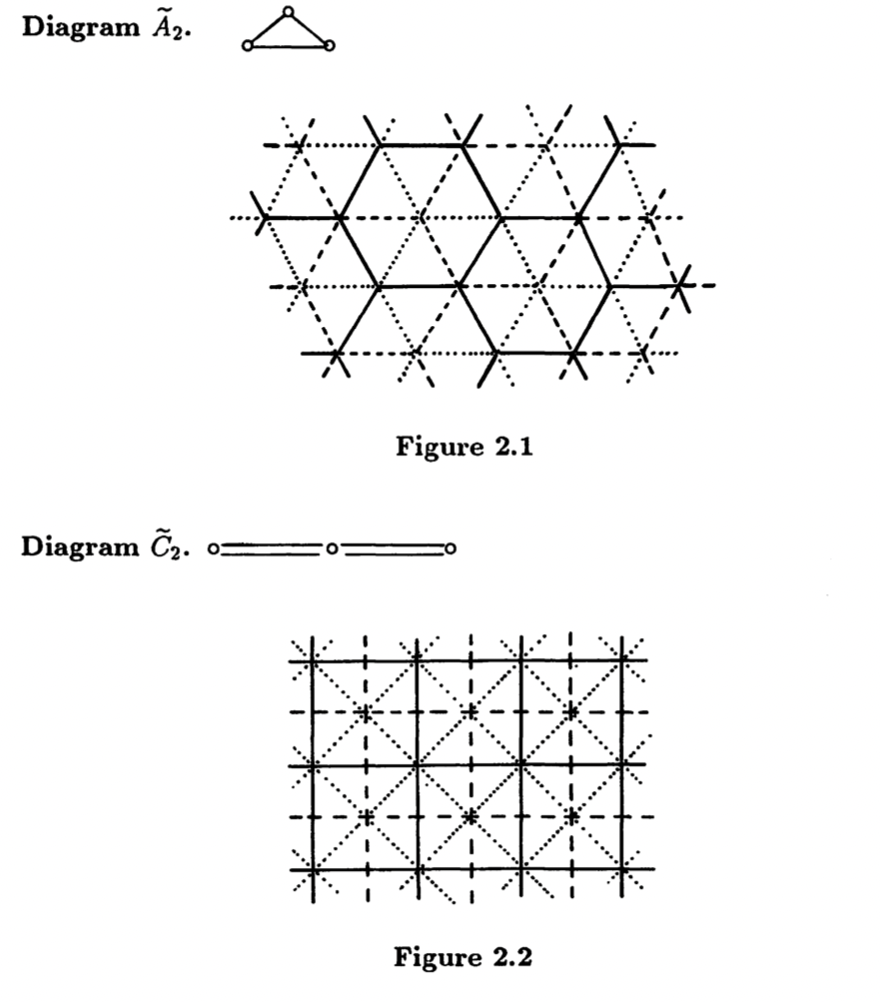
\includegraphics[scale=0.7]{Screenshot 2023-02-20 at 14.12.15.png}\\

\begin{lemma}
    The automorphism group of the Coxeter complex is isomorphic to the Coxeter group, and this acts simple-transitively on the set of chambers.
\end{lemma}

\begin{definition}
    A \ix{reflection r} of $W$ is a conjugate of the generators of $W$. The wall $M_r$ of a reflection $r$ is the set of simplicies in the Coxeter complex which is fied by $r$ when $r$ acts on the complex by left multiplication. Then $M_r$ is a subcomplex of codimension 1.
\end{definition}

\begin{theorem}
    There is a bijection between the set of reflections of a Coxeter group, and the set of walls in the corresponding Coxeter complex.
\end{theorem}

\begin{definition}
    A gallery $(c_0,...,c_k)$ \ix{crosses } $M_r$ if there is an $i$ such that $M_r$ interchanges $c_{i-1}$ and $c_i$. 
\end{definition}

\begin{lemma}
    \begin{enumerate}
        \item Any minimal gallery does not cross a wall twice.
        \item Every gallery from two alcoves $x$ and $y$ have the same parity of crossings of any wall.
    \end{enumerate}
\end{lemma}

\begin{definition}
    Each hyperplane splits an apartment into two half-apartments called \ix{roots}. If $\alpha$ is one root, we denote the other corresponding root by $-\alpha$. 
\end{definition}


\begin{definition}
    A set of alcoves is called \ix{convex} if any minimal gallery between two alcoves of the set lies entirely within the set. 
\end{definition}

\begin{proposition}
    \begin{enumerate}
        \item Roots are convex.
        \item Let $\alpha$ be a root, and let $x$ and $y$ be adjacent chambers with $x\in\alpha$ and $y\in -\alpha$. Then
        \[\alpha =\{c|d(x,c)<d(y,c)\}.\]
        \item There are bijections between the set of all reflections of a Coxeter group, the set of walls, and the set of pairs of opposite roots.
    \end{enumerate}
\end{proposition}

\begin{definition}
    A \ix{folding of W onto $\alpha$} is the map which fixes $\alpha$ and sends $-\alpha$ to $\alpha$ by relfecting across the the defining wall of $\alpha$. 
\end{definition}

\begin{proposition}
    Consider any chambers $x$ and $y$. Let $(x,x_1,...,x_{k-1},y)$ be a minimal gallery from $x$ to $y$. Define $\beta_i$ to be the root which contains $x_{i-1}$ and which does not contain $x_i$. Then the $\beta_i$ are all distinct, and this set is all the roots which contain $x$ but do not contain $y$. So in particular, $d(x,y)=k$ is the size of the set of roots containing $x$ but not containing $y$. 
\end{proposition}


\begin{proposition}
    Given two chambers $x$ and $y$, a third chamber $z$ lies on a minimal gallery from $x$ to $y$ if and only if it is contained within every root which also contains $x$ and $y$. 
\end{proposition}


Let $R$ be a residue. Now we can define a map, called proj$_Rw$, which maps $w$ to the unique chamber of $R$ closest to $w$. 


\begin{proposition}
    Given a residue $R$ and a chamber $x\in R$, for any chamber $w$ there is a minimal gallery from $x$ to $w$ which passes through proj$_Rw$. 
\end{proposition}

\begin{lemma}
    Residues are convex.
\end{lemma}

\begin{theorem}
    Given a gallery $\gamma$ of type $f$, $\gamma$ is minimal if and only if $f$ is reduced.
\end{theorem}


\subsection{Finite Coxeter complexes}

Now we assume that our group $W$ is finite, and so our Coxeter complex is also finite.

\begin{definition}
    The \ix{diameter}, diam$(W)$, of $W$ is the maximum distance between two chambers of the Coxeter complex. Two chambers are said to be \ix{opposite} if the distance between them is diam$(W)$.
\end{definition}

\begin{theorem}
    \begin{enumerate}
        \item diam$(W) = 1/2\ast |\{${roots of W}$\}|$. 
        \item Two chambers are contained in no common root if and only if they are opposite.
        \item For any given chamber, there is a unique opposite chamber.
        \item Any chamber lies on a minimal gallery between two opposite chambers.
    \end{enumerate}
\end{theorem}


\section{Buildings}

\begin{definition}
    Let $(W,S)$ be a Coxeter group with Coxeter matrix $M$, and let $I$ be an indexing set for the generators of $W$. A \ix{building of type M} is a chamber system $\Delta$ over $I$, such that each panel lies on at least two chambers, i.e every $\{i\}$-residue contains at least two elements. We also require a $W$-distance function
    \[\delta:\Delta\times \Delta \to W,\]
    such that if $f$ is a reduced word in $S$, then we have that $\delta(x,y)=s_f$ if and only if 
\end{definition}



\begin{example}
    Taking our $W$-distance function to be $\delta(x,y)=x^{-1}y$, Coxeter complexes are buildings.
\end{example}


Some key properties of bulidings are as follows:
\begin{enumerate}
    \item $\Delta$ is connected.
    \item $\delta$ is surjective.
    \item $\delta(x,y)=\delta(y,x)^{-1}$.
    \item $\delta(x,y)=s_i$ if and only if $x\neq y$ and $x\sim_i y$.
    \item For $i\neq j$, $i$- and $j$-adjacency are mutually exclusive.
    \item For chambers $x$ and $y$, if there is a gallery form $x$ to $y$ of type $f$, and $f$ is homotopic to $g$, then there is a gallery from $x$ to $y$ of type $g$. 
    \item A gallery if minimal if and only if its type if reduced.
    \item If there is a gallery of type $f$ from $x$ to $y$, and $f$ is reduced, then this gallery is unique.
\end{enumerate}

\begin{theorem}
    Any $J$-residue is a building of type $M_J$. 
\end{theorem}

\begin{theorem}
    Any isometry from a subset of $W$ into $\Delta$ can be extended to an isometry of $W$ into $\Delta$.
\end{theorem}

\begin{corollary}
    Any two chambers lie in a common apartment.
\end{corollary}

\begin{theorem}
    Apartments are convex.
\end{theorem}

\section{BN-Pairs}

\begin{definition}
    Let $G$ be a group. A \ix{Tits system} or \ix{BN-pair} of $G$ is a a pair of subgroups $B$, $N$ such that
    \begin{enumerate}
        \item $G=\langle B,N\rangle$
        \item $B\cap N$ is normal inside $N$ and $W=N\backslash B\cap N$ is a Coxeter group with generators $s_1,...,s_n$.
        \item If $w\in W$ and $s=s_i$, then $BsBwB\subset BwB\cup BswB$.
        \item For all $s=s_i$, $sBs\neq B$. 
    \end{enumerate}
\end{definition}


\begin{definition}
    We say that a group $G$ of automorphisms on a building $\Delta$ is \ix{strongly transitive} if 
    \begin{enumerate}
        \item $G$ is transitive on the sets of pairs of chambers with the same $W$-distance, and
        \item there exists an apartment $\Sigma$ whose stabiliser in $G$ is transitive on the apartments of $\Sigma$. 
    \end{enumerate}
\end{definition}

\begin{theorem}
    Let $G$ act strongly transitively on a thick building $\Delta$. Let $\Sigma$ be as above, and take $W$ to be the corresponding Coxeter group. Choose a chamber $c$ in $\Sigma$, and take $B=$stab$_
\end{theorem}



























\end{document}